\section{Sound Objects}
\label{soundObjects}

Sound Objects are objects on the score timeline that are primarily
responsible for generating score data.

The following are properties that all SoundObjects share.

\begin{description}
\item[Name]
Name of the Soundobject
\item[Subjective Duration]
The duration of the soundObject on the timeline (versus the duration of
the generated score within the soundObject, which may be different). How
the duration relates to the generated score contents is controlled by
the "Time Behavior" property.
\item[End Time]
Read-Only property that shows the end-time of the soundObject
\item[Time Behavior]
Selects how subjective time should be used on a soundObject. Options
are:

\begin{enumerate}
\def\labelenumi{\arabic{enumi}.}
\item
  Scale - The default option, stretches generated score to last the
  duration of the soundObject
\item
  Repeat - repeats generated score up to the duration of the soundObject
\item
  None - Passes the score data as-is (When using Time-Behavior of None,
  width of soundObject no longer visually corresponds to duration of the
  soundObject's score.)
\end{enumerate}
\end{description}

Sound Objects generate notes in the following manner:

\begin{itemize}
\item
  SoundObject generates initial notes
\item
  NoteProcessors are applied to the generated notes
\item
  Time Behavior is applied to the notes
\end{itemize}

When using a render start time other than 0.0, how soundObjects
contribute notes depends on if they support partial object rendering.
Normally, notes from all soundObjects which can possibly contribute
notes to the render (taking into account render start and render end)
are gathered and then if any notes start before the render start time
they are discarded as there is no way to start in the middle of a note
and to know exactly that it sounds as it should as blue's timeline only
knows about notes and not how those instruments render.

However, there are certain cases where blue soundObjects *can* know
about the instrument that the notes are generated for and can therefore
do partial object rendering to start in the middle of a note. This the
is the case for those soundObjects which generate their own instruments,
such as the AudioFile SoundObject, FrozenObject, the LineObject, and the
ZakLineObject. For those soundObjects, if render is started within the
middle of one of those, you will hear audio and have control signals
generated from the correct place and time.

\section{AudioFile}\label{audioFile}

Accepts NoteProcessors: no

Allows for quickly putting in a soundfile on the timeline.

\section{CeciliaModule}\label{ceciliaModule}

Accepts NoteProcessors: no, Supports TimeBehavior: no

\begin{quote}
\textbf{Note}

This SoundObject is unfinished and not enabled for normal use. This
information is left here for the future if the module is ever finished
and reenabled.
\end{quote}

The CeciliaModule is a soundObject that is meant to be compatible with
modules for the program Cecilia
(http://www.sourceforge.net/projects/cecilia), created by Alexandre
Burton and Jean Piche. The CeciliaModule is not as fully featured as
Cecilia itself as some features found in Cecilia do not make sense
within the context of blue.

One major advantage of the CeciliaModule is the ability to have as
manyinstances of a module on the timeline as one likes, all without one
worrying about variable name clashes or other issues. blue automatically
parses and renumbers instruments, ftables, and score statements so that
they do not interfere with other instances of the same module.

Cecilia modules require at least one modification before they are able
to run in blue, and also must adhere to a few more constraints of
design.

\textbf{Appending ``ftable'' in Instrument Definitions.}

Instruments are required to append the word ``ftable'' before any number
that is meant to be an ftable. For example:

\begin{verbatim}
        instr 1

        aout oscil 10000, 440, 1

        out aout, aout endin
      
\end{verbatim}

would have to become:

\begin{verbatim}
        instr 1

        aout oscil 10000, 440, ftable1

        out aout, aout endin
      
\end{verbatim}

The purpose of this is so that blue will know what ftable references
will need to be updated when blue reassigns ftable numbers.

\section{ClojureObject}\label{clojureObject}

ClojureObject

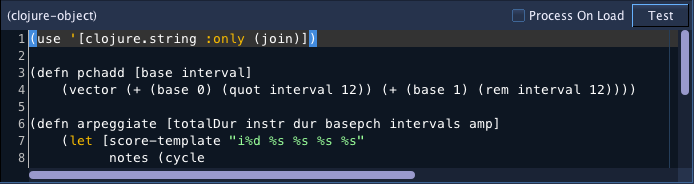
\includegraphics[width=1.00000\textwidth]{images/clojureObject.png}

Accepts NoteProcessors: yes

Allows using the \href{http://www.clojure.org}{Clojure} programming
language to generate score data. The Clojure interpreter is included
with Blue, so ClojureObjects are portable between systems without any
external dependencies. Users do not have to install anything further to
use this object, and the code will continue to function for the duration
of Blue's existence.

When writing your script to generate notes, assign the string value of
the notes to the symbol 'score'. Blue will then read in the value from
that variable and continue processing.

\begin{verbatim}
(def score "i1 0 2 3 4 5")
    
\end{verbatim}

The above example shows the simplest script and will generate a single
note. If the ClojureObject is set with a start time of 0 and a duration
of 2, then it will generate the following score:

\begin{verbatim}
i1  0.0 2   3   4   5
    
\end{verbatim}

\begin{verbatim}
(use '[clojure.string :only (join)])

(defn pchadd [base interval] 
    (vector (+ (base 0) (quot interval 12)) (+ (base 1) (rem interval 12))))

(defn arpeggiate [totalDur instr dur basepch intervals amp]
    (let [score-template "i%d %s %s %s %s"
          notes (cycle 
                    (map #(apply format "%d.%02d" (pchadd basepch %1)) 
                        (concat intervals (subvec intervals 1 (- (count intervals) 1)))))]
    (join \newline
        (map #(format score-template instr %1 dur %2 amp) 
            (range 0 totalDur dur) ; list that will limit the map
            notes))))

(def score (arpeggiate blueDuration 1 0.25 [8 0] [0 4 7] -12))
    
\end{verbatim}

The above example is taken from
blue/examples/soundObjects/clojureSoundObject.blue. This script defines
an apreggiate function, then calls that assigns the value to score.
Notice the use of blueDuration, a symbol that is automatically assigned
to the duration of the ClojureObject.

If the ClojureObject is set with a start time of 0 and a duration of 4,
then it will generate the following score:

\begin{verbatim}
i1  0.0 0.25    8.00    -12
i1  0.25    0.25    8.04    -12
i1  0.5 0.25    8.07    -12
i1  0.75    0.25    8.04    -12
i1  1.0 0.25    8.00    -12
i1  1.25    0.25    8.04    -12
i1  1.5 0.25    8.07    -12
i1  1.75    0.25    8.04    -12
i1  2.0 0.25    8.00    -12
i1  2.25    0.25    8.04    -12
i1  2.5 0.25    8.07    -12
i1  2.75    0.25    8.04    -12
i1  3.0 0.25    8.00    -12
i1  3.25    0.25    8.04    -12
i1  3.5 0.25    8.07    -12
i1  3.75    0.25    8.04    -12
    
\end{verbatim}

Blue processes soundObjects by going through each SoundLayer and
generating score for each object within each layer. This is useful to
know so that if you are using a ClojureObject that has utility functions
that you later use in other ClojureObjects, you should put that utility
ClojureObject on the first SoundLayer closest to the top, or at least on
a layer above all others that contain ClojureObjects.

Also to note, as a feature, Blue uses a single interpreter instance for
processing Clojure code. Therefore, if one ClojureObject has code
evaluated, the values from that code can be read by other objects. This
allows creating utility ClojureObjects. However, one can use stale
values (or values from another project even) if one is not careful to
always assign values in the project that require being set for this
particular project.

The following variables are avaialable from blue:

\begin{description}
\item[blueDuration]
Duration of the Clojure SoundObject
\item[blueProjectDir]
The location of the current project's directory. Includes path separator
at end.
\end{description}

There is a checkbox entitled "Process at Start". Selecting this option
will have the script of the ClojureObject run when a .blue project is
loaded. This is useful for scripts that act as library functions, but
themselves do not generate any notes. For example, you might define a
number of score generation utility functions in one ClojureObject that
has "Process at Start" enabled. Your other ClojureObject may then use
the functions from that ClojureObject Next time you load your project,
if that ClojureObject hasn't been run, your other ClojureObject will not
be able to be run either. If you are rendering from the beginning of a
project, this won't be an issue, but if you're starting work in the
middle of a project, you will need to evaluate that utility
ClojureObject at least once. You can either do a run from the start at
least once, use the "Test" button to have that evaluated, or use
"Process at Start" and have blue ensure it is loaded into the Clojure
interpreter when you load your projects.

Blue is able to load external .clj scripts, resolved from the
.blue/script/clojure or PROJECT\_DIR/script/clojure directory. For
example, if you use:

\begin{verbatim}
(use 'my.script)      
    
\end{verbatim}

This will try to load the script from
"/Users/me/.blue/script/clojure/my/script.clj" or
"/path/to/blueProject/script/clojure/script.clj".

\section{Comment}\label{comment}

Accepts NoteProcessors: no

Used to add comment text on the timeline and does not generate any
notes.

\section{External SoundObject}\label{externalSoundObject}

Accepts NoteProcessors: no

Allows you to write script within blue and execute an external program
on that script, bringing in generated notes back into blue. There is a
field for 'command line' as well as a text area for your script. When
this soundObject is called for generating it's notes, it will write the
text within the text area into a temp file and then use the
user-supplied 'command line' to execute on that temp file.

When blue runs the commandline, it defaults to appending the temp file's
name to the end of the commandline. For example, if you wrote a perl
script in the text area and used a commandline of "perl", then when blue
runs the command, it would be something like "perl
/the/path/to/the/tempFile". If you need to explicitly put the name of
the temp file somewhere else in the command line than the end, you can
use "\$infile" in your commandline. For example, if you needed something
like "myCommand somefileName -w -d -\/-some-other-flags" and had to have
it in that order, you could type "myCommand \$infile -w -d
-\/-some-other-flags" and blue will replace that \$infile with the temp
file's name instead of appending it to the end.

When designing your scripts that you will be using with external
programs, you should either set commandline flags to the program or
script your script in a way that it will write out to stdout(to the
screen), as that is what blue will capture and bring in as notes.

A second method for the external object was created for bringing in
score data after running the commandline as some programs (i.e. Cmask)
do not have any possible way to write directly to stdout. The process is
to use "\$outfile" in the commandline to pass in a filename to the
program. That \$outfile will be the name of a temp file that the
external program will write score data into. After the program is
finished, blue will open up that temp file, read in the score data, and
then remove the temp file. So, if your program needed a commandline of
something like "myProgram -i inputfilename -o outputfilename" and no
options for writing to screen, then you could use a commandline of
"myProgram -i \$infile -o \$outfile".

There is a test button that you may use to check to see that blue
properly brings in the generated notes.

This is a list of commandlines to use when using other programs with
blue and any notes that may concern other programs when being used with
blue. These commandlines assume that the programs being called are on
the system path. If not on the path, please append the full path to the
program before the program name.

\begin{description}
\item[CMask]
Homepage: \url{http://www.bartetzki.de/en/software.html} for the Linux,
Windows and old Mac builds,
\url{http://www.anthonykozar.net/ports/cmask/} for OSX Author: Andre
Bartetzki

Comandline to use:

\begin{verbatim}
cmask $infile $outfile
\end{verbatim}
\item[nGen]
Homepage: \url{http://mikelkuehn.com/index.php/ng} Author: Mikel Kuehn

Comandline to use:

\begin{verbatim}
ngen $infile $outfile
\end{verbatim}
\item[AthenaCL]
Homepage: \url{http://www.flexatone.org/athena.html} Author: Christopher
Ariza

Comandline to use:

\begin{verbatim}
python athenaPipe.py $infile
\end{verbatim}
\end{description}

Examples of the External SoundObject, as well as athenaPipe.py, can be
found in the blue/examples/soundObjects folder.

\section{GenericScore}\label{genericScore}

Accepts NoteProcessors: yes

Contains a block of Csound score text. The objective time within the
GenericScore starts at time 0, and notes within the genericScore are
written relative to 0. The start time of the GenericScore object within
the timeline will translate the score text's time, and the SoundObject's
time behavior will determine how the notes are processed relative to the
GenericScore's duration. For example, for the following score:

\begin{verbatim}
i1 0 1 2 3 4 5
i1 1 1 2 3 4 5
i1 2 1 2 3 4 5
  
\end{verbatim}

If this SoundObject is moved to start at time 2.0 with duration 6.0, the
generated score will be:

\begin{verbatim}
i1 2 2 2 3 4 5
i1 4 2 2 3 4 5
i1 6 2 2 3 4 5
  
\end{verbatim}

\begin{quote}
\textbf{Note}

Score blocks support only a subset of the Csound Score Syntax. Using "+"
in p2 and "." in pfields, as well as "\textless{}" and "\textgreater{}"
is supported.
\end{quote}

\section{Instance}\label{instanceObject}

Accepts NoteProcessors: yes

A SoundObject that points to a SoundObject in the SoundObject library.
The content of the SoundObject is not editable except by editing the
SoundObject in the library to which the instance is pointing to. If
editing the SoundObject in the library, all instances that point to that
SoundObject will be changed.

When clicking on an Instance object to edit it, the SoundObject from the
library will show its editor instead in the SoundObject edit area, but
it will be clearly marked that the user is currently editing a library
SoundObject and not an individual SoundObject.

The instance object is very useful if your work entails using many
variations of single source of material. For example, you can take a
SoundObject that represents a drum pattern, then make many Instances of
that pattern and add them to your project. If you want to later change
the base pattern, it will update everywhere that there are Instance
objects pointing to it.

Another example, if you have a SoundObject that represents a motive or
melodic fragment, you can put it into the SoundObject library, then make
10 instances of it, adding noteProcessors to do things like transpose or
get the retrograde, etc. Later, if you decide you want to change the
base material, you'd only have to edit it once within the library. All
Instance objects pointing to the changed object will be updated and will
maintain all of their transformations and relationships that were added
via NoteProcessors.

If you later decide that you want to work with the original material
where you have an Instance and want to break the link, replacing the
instance with a copy of the original to modify, you can convert the
Instance object to a GenericScore. To do this, you can use one of two
methods:

\begin{itemize}
\tightlist
\item
  Right-click the Instance object and choose "Convert to Generic Score"
\item
  Go the SoundObject Library, select the original and use "Copy", then
  select the Instance object and use "Replace with SoundObject in
  Buffer"
\end{itemize}

\section{JMask}\label{jmask}

Accepts NoteProcessors: yes

JMask is GUI score generating soundObject based on Andre Bartetzki's
\href{http://www.bartetzki.de/en/software.html}{CMask}. JMask currently
supports all features of CMask except field precision, though support
for this feature is planned. Users of JMask are encouraged to read the
CMask manual available at Andre Bartetzki's site to get familiar with
CMask concepts as they are represented 1:1 in JMask.

JMask builds on top of CMask's concepts and feature set by providing the
user a graphical way to edit parameter values, tables, masks, etc. Also,
by using JMask, the user's projects are guaranteed to run on all blue
installations, while using CMask from blue requires anyone opening and
using the project to have CMask installed on their system.

The following documentation for JMask will assume the user is familiar
with CMask and that the user has read through the CMask manual available
from the link above. The following will discuss how to use JMask,
covering how the CMask features are implemented in JMask and how to work
with the user interface. Over time, this manual entry for JMask will
attempt to grow to be self sufficient and not require knowledge of
CMask, but for now familiarity with CMask is suggested.

\subsection{Overview}\label{jmaskOverview}

A single JMask object is equivalent to one CMask field. A single JMask
object holds a collection of Parameters, one for each pfield to be
generated in the score. Each of the Parameter types in CMask is
available in JMask:

\begin{longtable}[]{@{}ll@{}}
\caption{Parameter Types}\tabularnewline
\toprule
Type & Description\tabularnewline
\midrule
\endfirsthead
\toprule
Type & Description\tabularnewline
\midrule
\endhead
Constant & Generate the given value when generating values for
notes\tabularnewline
Item List & Generates values from a list of values given by the user.
Options for generation include cycling through the list (cycle), going
backwards and forwards through the list (swing), going through the list
in random order using all values once before repeating (heap), and
choosing a random list item (random).\tabularnewline
Segment & Generates values along a user-defined line.\tabularnewline
Random & Generates a random value.\tabularnewline
Probability & Generates a randomized value that is weighted by the given
probability type and the configuration of the parameters of that
probability type.\tabularnewline
Oscillator & Generates values that oscillate in a given period using
different user-chosen shapes.\tabularnewline
\bottomrule
\end{longtable}

Beyond the Parameters, JMask supports the three modifier types found in
CMask: Masks, Quantizers, and Accumulators. Certain parameters support
different modifiers, and their support by paramater type is listed
below:

\begin{longtable}[]{@{}llll@{}}
\caption{Parameter Modifier Support}\tabularnewline
\toprule
Type & Supports Mask & Supports Quantizer & Supports
Accumulator\tabularnewline
\midrule
\endfirsthead
\toprule
Type & Supports Mask & Supports Quantizer & Supports
Accumulator\tabularnewline
\midrule
\endhead
Constant & No & No & Yes\tabularnewline
List & No & No & Yes\tabularnewline
Segment & No & Yes & Yes\tabularnewline
Random & No & Yes & Yes\tabularnewline
Probability & Yes & Yes & Yes\tabularnewline
Oscillator & Yes & Yes & Yes\tabularnewline
\bottomrule
\end{longtable}

JMask also supports the use of a seed value. When enabling the use of
seeding, the seed value will be used to initialize the pseudo-random
number generator used in randomized operations. This allows the user to
set a seed and get consistently reproducible results. The default is to
use the system time to seed the random number generator, thus giving
different results each render.

\subsection{Using the JMask Interface}\label{jmaskInterface}

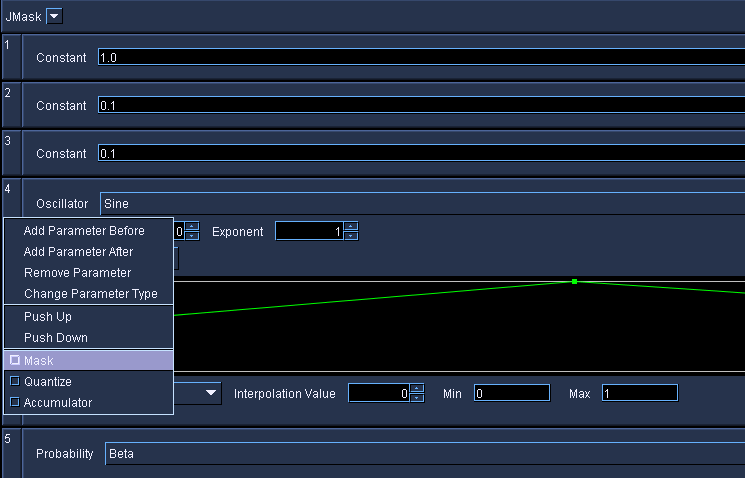
\includegraphics{images/jmask.png}

The JMask SoundObject Editor allows for viewing the editors for all of
the assigned parameters. Parameters are each set to generate values for
one pfield. On the top side of each row is the Parameter Edit Panel.
This panel shows a number at the top that corresponds to what pfield
this parameter will generate values for, as well as the field name. To
change things about the Parameter, right-click the panel to show a popup
menu as shown in the image above. The options are described below:

\begin{description}
\item[Add Parameter Before]
Create a new Parameter and insert it before the Parameter clicked on by
mouse. When this option is selected, a dialog will appear with a
dropdown of options of what type of Parameter to add.
\item[Add Parameter After]
Create a new Parameter and insert it after the Parameter clicked on by
mouse. When this option is selected, a dialog will appear with a
dropdown of options of what type of Parameter to add.
\item[Remove Parameter]
Remove this Parameter. Will not be allowed if trying to edit parameters
1-3 as JMask requires a minimum of 3 pfields.
\item[Change Parameter Type]
Choose a different type of Parameter and replace the current one with
the selected one. Any edits from the old Parameter will be lost once a
new parameter type is chosen.
\item[Push Up]
Move the selected Parameter to before the previous Parameter. Example:
Push up parameter at pfield 5 to pfield 4, moving what was previously at
4 to 5.
\item[Push Down]
Move the selected Parameter to after the next Parameter. Example: Push
down parameter at pfield 4 to pfield 5, moving what was previously at 5
to 4.
\item[Mask]
Enable/disable using a Mask with this parameter. If enabled, the Mask
editor will appear, and if disabled, the Mask editor will disappear.
This menu option will not show for those Parameters that do not support
Masks.
\item[Quantizer]
Enable/disable using a Quantizer with this parameter. If enabled, the
Quantizer editor will appear, and if disabled, the Quantizer editor will
disappear. This menu option will not show for those Parameters that do
not support Quantizers.
\item[Accumulator]
Enable/disable using an Accumulator with this parameter. If enabled, the
Accumulator editor will appear, and if disabled, the Accumulator editor
will disappear. This menu option will not show for those Parameters
which do not support Accumulators.
\end{description}

Beyond the basics of moving around Parameters, adding new ones, and
choosing whether to enable Masks, Quantizeres, and Accumulators, one can
also choose to show/hide Parameters by using the popup menu that appears
when choosing the down arrow button in the JMask title bar, as shown in
the screenshot below.

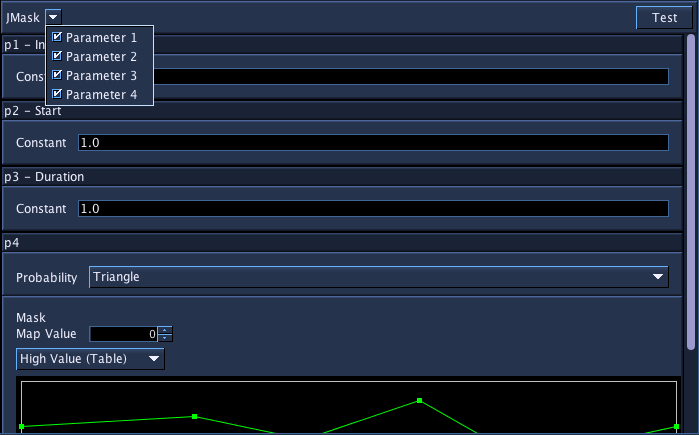
\includegraphics{images/jmask2.png}

To edit the field name, double click the Parameter Edit Panel. A dialog
will appear where you can modify the field name, as shown below:

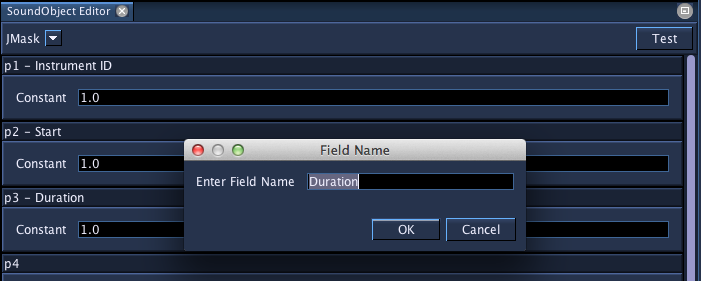
\includegraphics{images/jmask_field_name.png}

Beyond these basics for working with the Parameters in general, each
Parameter type has its own editor, each customized for the values and
options allowable for each Parameter. Currently, documentation is
omitted for each Parameter's GUI as they correspond in feature and
parameters as CMask, and the user is encouraged to consult the CMask
manual for more information on editing each Parameter.

\section{LineObject}\label{lineObject}

Accepts NoteProcessors: no

Line Object

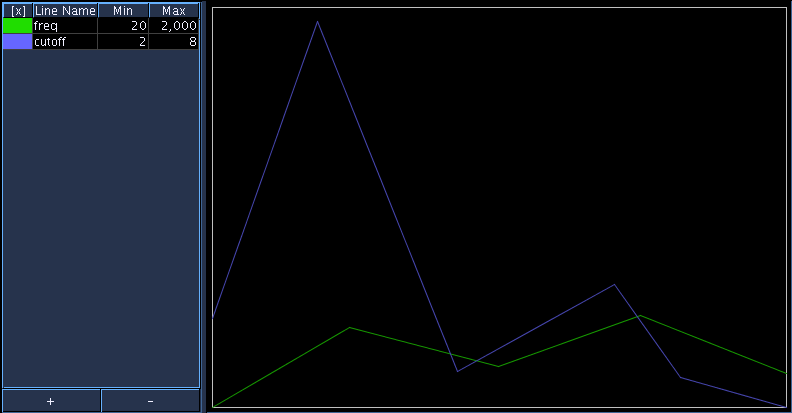
\includegraphics{images/lineObject.png}

Add and graphically edit global k-rate signals.

Use the bottom + and - buttons to add/remove lines.

Use the table to select a line. After selecting a line, you can edit the
points by dragging them, add points by clicking where you want the new
point, and remove points by rt-clicking them.

Use the table to edit the name of the signal, as well as the max and min
values (need to be floating point values). For editing the color of the
line, double-click the color box to the left of the lineName. A color
selection dialog will appear for the user to choose their desired color.

The name of the signal will be prepended with "gk" when outputing a
signal, i.e. a line name of "cutoff" will become "gkcutoff".

\subsection{ObjectBuilder}\label{objectBuilder}

Accepts NoteProcessors: Yes

This SoundObject allows users to build their own SoundObjects by using
the same widgets and features as the
\protect\hyperlink{blueSynthBuilder}{BlueSynthBuilder} for creating user
interfaces, as well as using either Python script or External Script for
the score generation. When generating score, the script has token values
replaced by values from the user interface before generating. The
scripts generated in the same manner as the
\protect\hyperlink{pythonObject}{PythonObject} and as the
\protect\hyperlink{externalSoundObject}{ExternalObject} .

Note: The code completion feature using ctrl-shift-space for values from
the UI that is available in BlueSynthBuilder is also available in this
SoundObject.

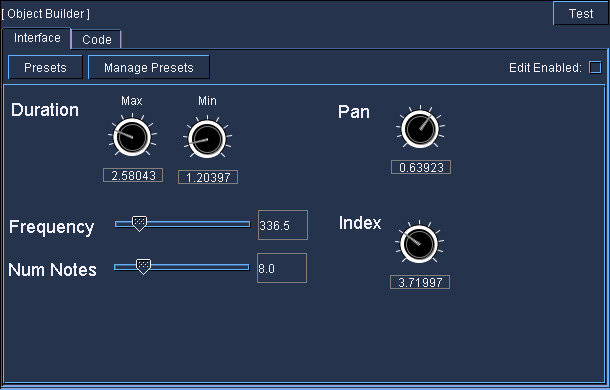
\includegraphics{images/objectBuilderUI.png}

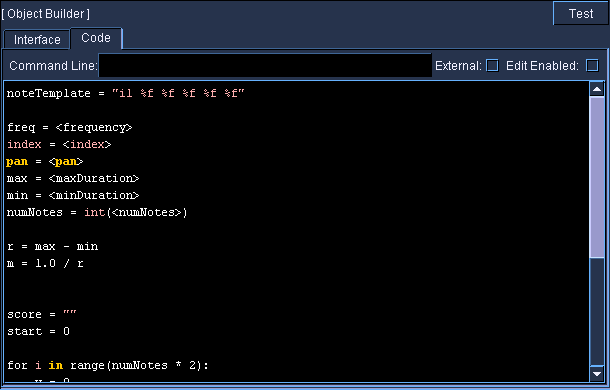
\includegraphics{images/objectBuilderCode.png}

\subsection{PatternObject}\label{patternObject}

Accepts NoteProcessors: yes

Pattern Object

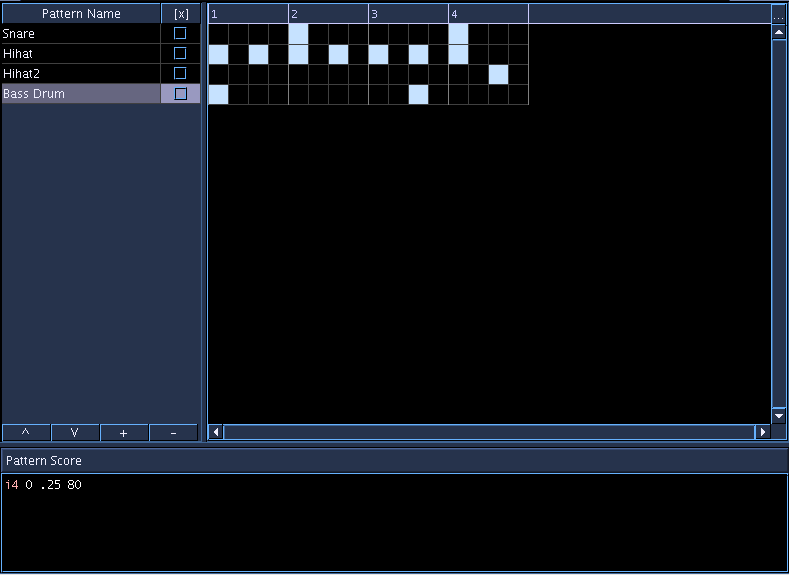
\includegraphics{images/patternObject1.png}

The PatternObject is pattern-based score editor, based on the author's
previous project "Patterns". It is a flexible pattern-oriented score
editor, useful for musical ideas which are pattern based, such as drum
parts or minimalist-style musical ideas.

For the general workflow of using the PatternObject, users will liked
likely want to:

\begin{enumerate}
\def\labelenumi{\arabic{enumi}.}
\item
  Setup the PatternObject Properties (number of beats and subdivisions)
\item
  Add Patterns, giving each pattern a name to help identify what the
  pattern is for
\item
  Edit each Pattern's score
\item
  Visually edit the PatternObject score
\end{enumerate}

The PatternObject's Time Properties can be modified by clicking on the
button in the upper-right corner of the editor. Clicking the button will
hide or show the properties panel on the right, as shown below:
PatternObject - Properties PatternObject - Properties

\begin{quote}
\textbf{Note}

Editing the time values will clear out any pattern triggers that the
user has entered. It is recommended that one first decide the pattern
time properties before working with the PatternObject.
\end{quote}

To add Patterns to the PatternObject, use the "+" button on the bottom
of the left hand section. Double-clicking the name of the pattern name
will allow editing of the name, and clicking on the {[}x{]} box will
allow for muting the Pattern. Clicking on the Pattern in the table will
also bring up it's score in the area below.

The Pattern's score is standard Csound SCO text, with the same features
supported as by the GenericScore SoundObject. Each score should be
started from time zero. The Pattern's score should be set such that its
score's total duration fits within the time of the subDivision. For
example, if the properties set for the PatternObject's time values are 4
beats and 4 subdivisions, each beat is 1.0 in duration (corresponds to
p3 value of a note) and thus a single subdivision in this case would be
equivalent to .25. Scores shorter or longer than the subdivision length
are allowed, but one should be aware that the resultant score may or may
not longer than what is visually represented on the PatternObject score.

The PatternObject score is visually edited by click on squares which
correspond to subdivisions of the beat. For example, if a Pattern's
score is .25 in total duration, and the time value of the PatternObject
is set to 4 and 4, then clicking a square would be to insert a 16th note
in a score.

To add to the PatternObject score, simply click on the square where one
wishes to have a Pattern triggered. To remove, simply click on a
selected square. The user can also click and drag to add or remove
mutliple triggers.

\begin{itemize}
\item
  Users may be surprised at the generated score if time behavior is not
  set to None(while others may prefer to use Scale, which is the
  default). Please be mindful of this, especially when using
  PatternObjects and the SoundObject library, where the default for
  creating instances of SoundObjects is to have Time Behavior of Scale
  on the Instance SoundObject.
\item
  When the PatternObject is used with a Scale time behavior, you may not
  get the results you think you will get if the pattern is not filled in
  in the last subdivision of the beat. When blue goes to generate a
  score for a soundObject, with a scale time behavior, the score is
  first generated, then scaled to the duration of the soundObject. So,
  if you're pattern has empty subdivisions and you're expecting there to
  be a space at the end of your pattern, when you go to generate the
  CSD, the space won't be there.

  To get around this, you may want to use a time behavior of None, or
  you may want put in a "ghost note" in a Pattern layer, using a note
  like:

\begin{verbatim}
i 10000 0 .25
    
\end{verbatim}

  Where 10000 is not an instrument in use in your project. Then you can
  put in a trigger for this pattern in the last subdivision. What will
  happen is that blue will process the score with this note's time and
  thus will generate with this out to the CSD, but Csound will ignore
  the note.

  When the PatternObject is set to use a time behavior of Repeat, the
  same situation can occur as when using Scale if a Repeat Point is not
  set, as the default for Repeat when no repeat point is set is to take
  the generated score and repeat it after the duration of the last note.
  To prevent this, either use the ghost note technique above or set a
  repeat point.
\end{itemize}

\section{PianoRoll}\label{pianoRoll}

Accepts NoteProcessors: yes

Piano Roll - Notes

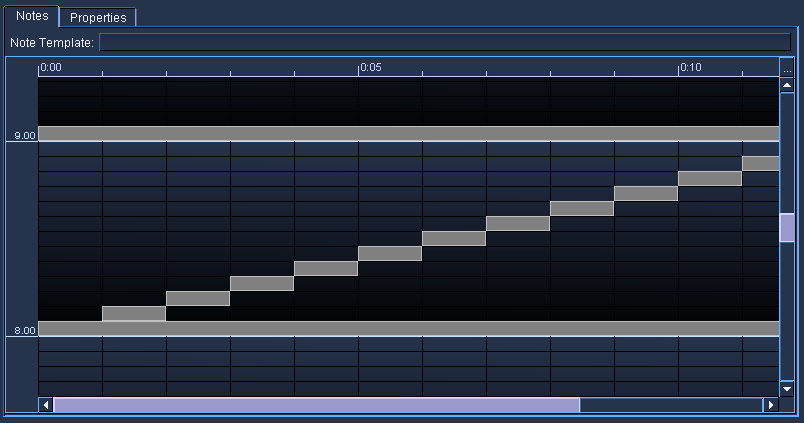
\includegraphics[width=1.00000\textwidth]{images/pianoRoll_notes.png}

The PianoRoll SoundObject is a graphical tool to enter in notes,
commonly available in many MIDI sequencer environments. This PianoRoll
is unique in that it is Microtonal: it supports loading any
\href{http://www.huygens-fokker.org/scala/}{Scala} scale file and
editing of notes adapts to that scale. For example, in the picture
above, the scale loaded is a Bohlen-Pierce scale with 13 tones to the
tritave. The PianoRoll above has adapted to that scale to show 13 scale
degrees per octave of its editor. The generated notes can output values
as either frequency or PCH notation (octave.scaleDegree). But don't
worry, if you're not interested in alternate tunings, the PianoRoll is
set by default to use 12-TET tuning, the "standard" tuning system in use
today.

The PianoRoll uses Note Template strings as a way to maintain
flexibility and be able to handle the open-ended nature of Csound's
instruments. Since the user who builds the instrument designs what each
pfield will mean(besides p1, p2, and p3), the Note Template string
should be made to match the instrument the user wants to use the
PianoRoll with. When the note is generated, certain special text values
(those enclosed in \textless{} and \textgreater{}) will be replaced by
values unique to the note.

For example, the following Note Template string:

\begin{verbatim}
      i<INSTR_ID> <START> <DUR> <FREQ> 0 1 1
    
\end{verbatim}

Will have the \textless{}INSTR\_ID\textgreater{} replaced with the value
set in the Piano Roll properties, \textless{}START\textgreater{}
replaced the start time for the note, \textless{}DUR\textgreater{}
replaced with the duration of the note, and
\textless{}FREQ\textgreater{} replaced with either a frequency or PCH
value, depending on how the Piano Roll is configured in its properties.
The other values will pass through as part of the note.

\begin{quote}
\textbf{Warning}

Caution should be used when creating a Note Template string to make sure
that there are enough spaces allowed between replacement strings. For
example, the following:

\begin{verbatim}
i<INSTR_ID> <START> <DUR> <FREQ> <FREQ> 0 1 1
      
\end{verbatim}

would result in:

\begin{verbatim}
i1 0 2 440 440 0 1 1
      
\end{verbatim}

while the following:

\begin{verbatim}
i<INSTR_ID> <START> <DUR> <FREQ><FREQ> 0 1 1
      
\end{verbatim}

which does not have proper space between the two
\textless{}FREQ\textgreater{} tags, results in:

\begin{verbatim}
i1 0 2 440440 0 1 1
      
\end{verbatim}
\end{quote}

The PianoRoll requires a bit of configuration before using. The
properties page below shows the properties that should be configure
before using the actual note drawing canvas.

Piano Roll - Notes - Properties

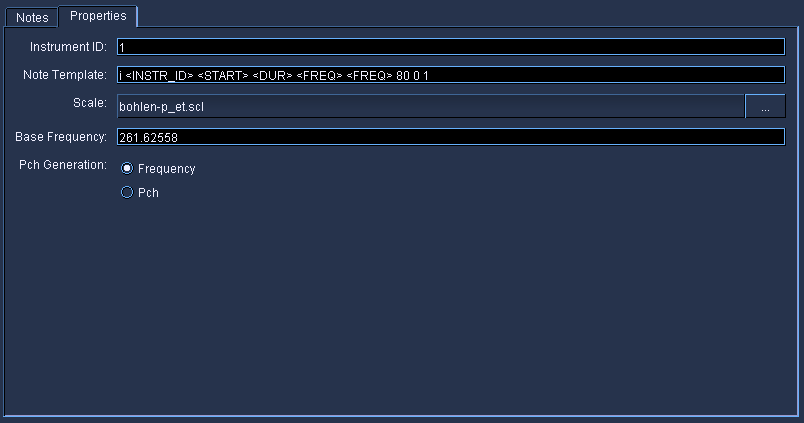
\includegraphics[width=1.00000\textwidth]{images/pianoRoll_properties.png}

\begin{description}
\item[Instrument ID]
Instrument name or number to be used when replacing
\textless{}INSTR\_ID\textgreater{} in Note template strings.
\item[Note Template]
The default note template when inserting notes. Notes make a copy of
this template string when created and edits to the note's string stay
with the note. Generally, you'll want to create a template string that
will match the instrument this PianoRoll will be used with.
\item[Scale]
The scale used with this PianoRoll. The PianoRoll defaults to a 12-TET
scale, the "standard" scale in use in Western classical and popular
music. Pressing the button labeled "..." will open a file browser for
selecting Scala scales to use in place of the default. After selecting a
scale, the PianoRoll will adjust the note canvas for the number of scale
degrees the newly selected scale contains.
\item[Base Frequency]
The base frequency of the scale for octave 8 and scale degree 0 (8.00).
Defaults to C below A440.
\item[Pch Generation]
Selects how the notes will generate their value to be used when
replacing the \textless{}FREQ\textgreater{} tag value in a note
template. The options are:

\begin{description}
\item[Frequency]
The value of the note's pitch expressed in terms of frequency in hertz.
This value is calculated using the chosen Scale for the PianoRoll.
\item[blue PCH]
Value of note expressed in blue PCH, a format similar to Csound PCH but
differs in that it does not allow fractional values. Values are
generated as "octave.scaleDegree" i.e. "8.22" would be octave 8 and
scale degree 22 in a scale that has 23 or more notes, or would wrap
around as it does in Csound PCH. If the scale had 12 scale degrees, the
"8.22" would be interpreted as "9.10". blue PCH is allowed as an option
to be used with blue PCH note processors and then to be used with the
Tuning NoteProcessor.
\item[MIDI]
When this Pch Generation method is chosen, a MIDI note value (0-127, 60
= Middle-C) is used for \textless{}FREQ\textgreater{} and the chosen
Scale will not be used. The display for the editor will automatically
switch to show octaves and notes for standard MIDI scale values. Using
MIDI note values is useful for instruments that exepct MIDI note values
such as the fluidsynth opcodes as well as midiout.
\end{description}
\end{description}

Piano Roll - Notes - Time Options

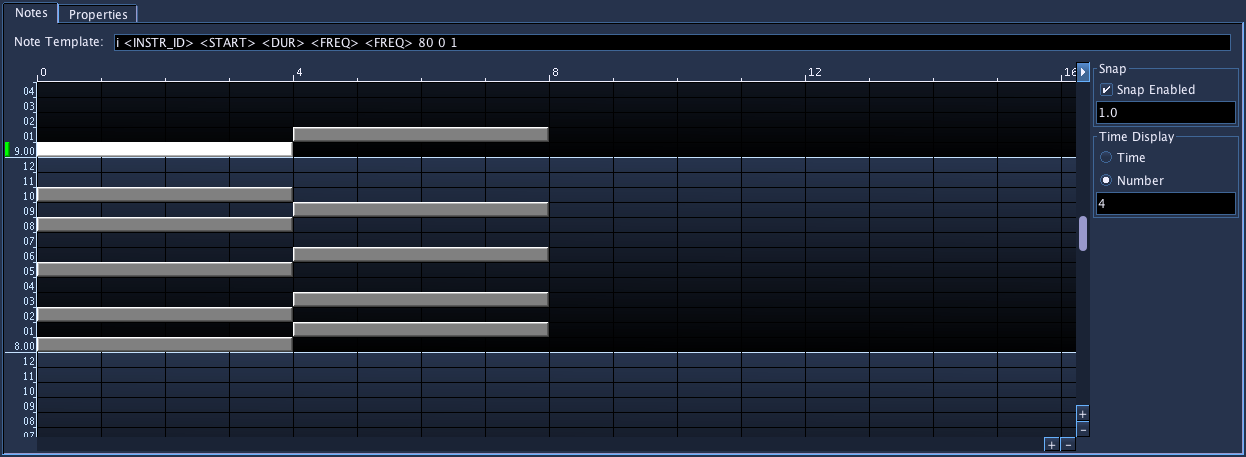
\includegraphics[width=1.00000\textwidth]{images/pianoRoll_notes_snap.png}

The Time Options in the PianoRoll are accessed and behave very much in
the same manner as those that are in the main timeline. The button
labelled "..." in the upper right corner of the PianoRoll canvas will
open and close the panel on the right that contains the properties.

\begin{description}
\item[Snap Enabled]
Enables snapping behavior on the timeline. If enabled, vertical lines
will be drawn at snap points, set by the value below it. In the
screenshot above, the snap is enabled and set to every 1.0 beats.
\item[Time Display]
Controls how the time in the time bar above the PianoRoll canvas will
display. The time value will show as time, while Number display will
display as integers. The number below show how often to put a label. In
the screenshot above, the Time Display is set to show a label in units
of time and at every 5.0 seconds.
\end{description}

To enter notes, hold down the shift key and press the left mouse button
down on the canvas. A note will be entered where you pressed and will be
set to resize as you move the mouse around. When you finally release the
mouse, the note will be finished entering.

After that, you can select notes by clicking on them or drag and
selecting notes by marquee. You can also press the shift key and click
on notes to add to the currently selected notes. You can then drag the
notes around by click a selected note and dragging. To resize a note,
select a single note, and after hilighted, move the mouse to the right
edge of the selected now, and then click and drag.

To remove a note or notes, select the notes, then press the del key.

To cut or copy a note, select a single note (only one note in the buffer
is currently supported), then press ctrl-x or ctrl-c to cut or copy,
respectively.

To paste, ctrl-click on the PianoNote canvas. (This is the same behavior
as pasting soundObjects on the main score timeline.)

To edit a note's template, select a single note. After selecting a note,
the text field for editing the note's template text will be enabled.
Here you can then edit the note's values.

\begin{quote}
\textbf{Note}

See the example .blue file in the blue/examples/soundObjects folder.
\end{quote}

\subsection{PolyObject}\label{polyObject}

Accepts NoteProcessors: yes

A timeline object that acts as a container for other SoundObjects.
PolyObjects can also be embedded within each other.

\begin{quote}
\textbf{Tip}

On the root timeline, rt-click on a soundLayer and select "Add new
PolyObject". You should have added a new PolyObject to the timeline. Now
either double-click or rt-click on the PolyObject and select "Edit
SoundObject". You should now be within the PolyObjects timeline, and the
button which says {[}root{]} should now have another button next to it
that says {[}PolyObject{]}. Now try adding a few soundLayers and a few
GenericScore Objects. Now click on {[}root{]}. You have now returned to
the root timeline. Here you should see the PolyObject you've edited. Now
you can scale the object you've created and all of the objects held
within will scale together as a group.
\end{quote}

\section{PythonObject}\label{pythonObject}

Accepts NoteProcessors: yes

Allows for using of the Python programming language to generate score
data, using the Jython interpreter to interpret Python scripts. You may
add your own python classes to the library for use with "import"
statements by adding them to your BLUE\_HOME/pythonLib folder. Included
with blue is Maurizio Umberto Puxeddu's pmask, as well as Steven Yi's
Orchestral Composition library, found in Blue's application directory
under blue/pythonLib.

After writing your script to generate notes, assign the string value of
the notes to the variable 'score'. Blue will then read in the value from
that variable and continue processing.

\begin{verbatim}
temp = ""

for i in range(4):
  temp += "i1 %d 1 %s %s\n"%(i, "8.0" + str(i), 80)

score = temp
    
\end{verbatim}

The above example script will generate four notes at ascending half
steps. If the PythonObject is set with a start time of 0 and a duration
of 2, then it will generate the following score:

\begin{verbatim}
i1  0.0 0.5 8.00    80
i1  0.5 0.5 8.01    80
i1  1.0 0.5 8.02    80
i1  1.5 0.5 8.03    80
    
\end{verbatim}

Blue processes soundObjects by going through each SoundLayer and
generating score for each object within each layer. This is useful to
know so that if you are using a PythonObject that has utility functions
that you later use in other PythonObjects, you should put that utility
PythonObject on the first SoundLayer closest to the top, or at least on
a layer above all others that contain PythonObjects.

Also to note, as a feature, Blue uses a single interpreter instance for
processing python code. Therefore, if one PythonObject has code
evaluated, the values from that code can be read by other objects. This
allows creating utility PythonObjects. However, one can use stale values
(or values from another project even) if one is not careful to always
assign values in the project that require being set for this particular
project.

The following variables are avaialable from blue:

\begin{description}
\item[blueDuration]
Duration of the Python SoundObject
\item[blueProjectDir]
The location of the current project's directory. Includes path separator
at end.
\end{description}

There is a checkbox entitled "Process at Start". Selecting this option
will have the script of the PythonObject run when a .blue project is
loaded. This is useful for scripts that act as library functions, but
themselves do not generate any notes. For example, you might define a
number of score generation utility functions in one PythonObject that
has "Process at Start" enabled. Your other PythonObjects may then use
the functions from that PythonObject. Next time you load your project,
if that PythonObject hasn't been run, your other PythonObjects will not
be able to be run either. If you are rendering from the beginning of a
project, this won't be an issue, but if you're starting work in the
middle of a project, you will need to evaluate that utility PythonObject
at least once. You can either do a run from the start at least once, use
the "Test" button to have that evaluated, or use "Process at Start" and
have blue ensure it is loaded into the python interpreter when you load
your projects.

\subsection{RhinoObject}\label{rhinoObject}

Accepts NoteProcessors: yes

Allows for the use of the JavaScript programming language to create
score data. uses the Rhino interpreter to interpret JavaScript scripts.

After writing your script to generate notes, you'll have to bring back
into blue by assigning the variable 'score' the text string of the
generated javaScript score.

\begin{verbatim}
[code for generating score]
...
         
score = myScoreGenerator();
\end{verbatim}

(where myScoreGenerator() is a function that will generate Csound SCO)

\section{Sound SoundObject}\label{sound}

Accepts NoteProcessors: no

Inline instruments. When experimenting with sounds, or if you're going
to make a soundEffect and not a whole composition, it might be tedious
to go and make an instrument and then have to edit score information.
This object is here so that you can add instruments directly to the
timeline. What is generated is a minimal i-statement that corresponds to
the sound soundObject's bar on a timeline. This abstracts a concept of
working with the sound itself instead of through the level of time of a
note.

\section{Tracker}\label{tracker}

Accepts NoteProcessors: yes

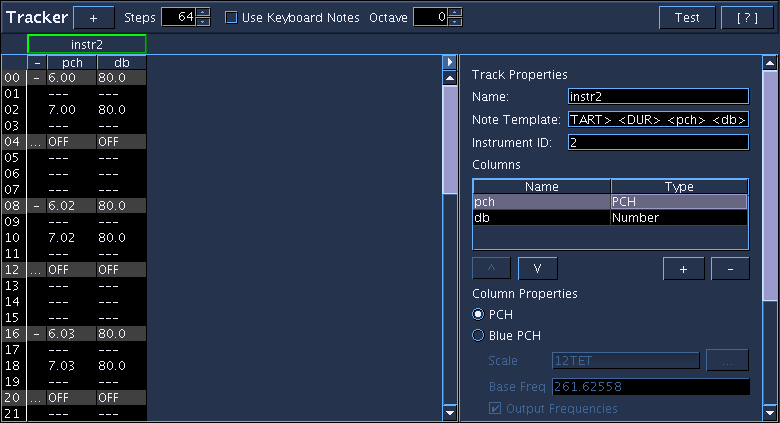
\includegraphics{images/tracker.png}

The Tracker SoundObject is a table-based tool to enter in patterns of
notes using the Tracker paradigm but in a way specific to Csound SCO
work. Each Tracker is organized in vertical Tracks of n number of steps
where n is configurable by the user (defaults to 64 steps). Notes are
entered into each Track with Tracks being configurable as to what
parameters (columns) to use. Unique to the blue Tracker SoundObject is
the support for microtonal scales using Scala scale files as well as
support for Csound's Tied-Notes feature.

The interface consists of three main areas: the top tool bar, the main
tracking area, and the track properties editor.

The top tool bar has a "+" button which adds new tracks to the Tracker,
a Steps entry widget to enter in the number of steps the Tracker should
have, a toggle for using Keyboard Note mode (see below for more
information), an Octave entry widget to determine the relative octave
for the Keyboard Note mode, a Test button to see what the generated
score will be for the Tracker, as well as a help button that opens up a
quick reference sheet for keyboard shortcuts.

The main tracking area is where all of the score work is done to enter
and modify notes. More information about note entry and modification is
available below in the section "Entering in Notes".

The last interface area is the track properties editor. The track
properties editor is held in a collapsible pane and when the tracker
editor initially loads it will be collapsed. To open up the track
properties, at least one track needs to be added to the tracker. Once
one track exists, click the small button above the right scroll bar to
open and close the track editor properties. More information on using
the properties editor follows below in the section "Settings Things Up".

When the Tracker Object is edited it is completely blank. To start,
click the "+" button to add as many tracks as you would like to use.
After adding the number of tracks you'd like to use you will need to
configure the track to work with your Csound instruments. Open up the
track properties editor using the "\textless{}" toggle button above the
right scroll bar. Afterwards, select a track by clicking the name panel
above a track. Selecting a track will populate the track properties
editor as well as hilight the name panel with a green border. A track's
properties consist of a Name, Note Template, Instrument ID, and Columns;
descriptions of the values are listed below.

\begin{description}
\item[Name]
The name property is used only for reference; editing the name changes
the title shown on the name panel and is for the user's reference.
\item[Note Template]
The note template is used when generating the notes for the track. Items
in the template that are within \textless{} and \textgreater{} tags will
be replaced by values either from the Tracker (START and DUR), the
Instrument ID (INSTR\_ID) or values from the columns, using the column's
name as a key (i.e. if a column is called "space", when generating a
note for the track, any value in the space column will replace the
\textless{}space\textgreater{} text in the note template). Note
templates will generally follow the form "i
\textless{}INSTR\_ID\textgreater{} \textless{}START\textgreater{}
\textless{}DUR\textgreater{}" and then have tag keys for each column for
the track.
\item[Instrument]
Instrument name or number to be used when replacing
\textless{}INSTR\_ID\textgreater{} in Note template strings.
\item[Columns]
Each track has a minimum of one configurable column (the tied-note is a
feature of all tracks and is not a part of this editor) and is
user-configurable to add as many columns as the user needs for the
values to use in their notes for their instruments. Columns are added
and removed using the Columns table and can be organized by pushing up
and down in the table which will move their order left and right in the
main tracking area. To edit the name of the Column, use the Columns
table to edit the name of the column.

Each Column also has a type. The type information is used by the tracker
when entering data to verify that the data being input is of that
column's type, as well as used when using shortcuts to manipulate data
in that column.

\begin{description}
\item[PCH]
Csound PCH format. Entering data will verify that data is in the
octave.pitch format. Using the increment and decrement value shortcuts
will propertly add or subtract one to pitch value, i.e. incrementing the
value of 8.11 will result in 9.00.
\item[blue PCH]
The blue PCH format is like the Csound PCH format except that the pitch
part is always a whole number integer and is the scale degree of the
selected Scale. A valid value in Csound PCH such as 8.01 is not valid in
Blue PCH as 01 is not an integer (the equivalent in blue PCH would be
8.1).

Using blue PCH allows for using Scala scale files to do microtonal
tracking. To choose a Scala scale, use the "..." button to open up a
file selector to choose a Scala scale. Afterwards, enter in the base
frequency for the scale (the default is 261.62558 or middle-c). The
"output frequencies" checkbox will determine how the values entered into
this column will be interpreted. By default, "output frequencies" is
enabled, meaning when the tracker goes to generate notes, it will take
the blue PCH values that are entered and convert them to a frequency
value in hertz. If you deselect this option, the tracker will pass the
blue PCH value out. This option should generally be left enabled unless
the user is planning to do further operation on the pch values via
NoteProcessors that work with blue PCH.

Using blue PCH, data will be verified on entry and increment/decrement
value options will work in the same way as for PCH.
\item[MIDI]
MIDI will limit the values entered to whole number integers from 0-127.
Using the increment and decrement value shortcuts will add or subtract 1
to the value.
\item[String]
The String type allows the user to input any value they want. No
verification is done on entry and the increment/decrement value
shortcuts will have no effect.
\item[Number]
The Number format will limit the values entered to only numbers. Values
can be further restricted to a given range as well as to only use whole
number integers. Using the increment and decrement value shortcuts will
add or subtract 1 to the value.
\end{description}
\end{description}

Entering in data into the tracker is much like entering data into any
other table, though learning the keyboard shortcuts will vastly speed up
entering and modifying data. To begin click anywhere on a track where
you would like to add a note. Now, begin typing to enter in a value for
that note, then press enter when you are finished. Depending on the type
of column you have configured, blue will verify that the data entered is
allowable and if so it will save that data to the note. If the value is
not allowable, the cell will become hilighted in red and will require
you to either fix your input to be valid or press esc to cancel entering
in data.

When entering in data for a new note, the first time you enter in
information for a column in the note's row, it will not only enter in
the data for the column, but also copy values for all other columns from
the first note that exists previous to the note being edited. If there
is no notes entered, some default settings will be used based on the
column type.

Like other tracker systems, the duration of a note entered will last as
long as until either the next entered note, the end of the pattern, or
until an OFF note is encountered. So, for example, if a note is entered
in step 0 and step 2, the duration of the first note will last 2 steps
while the second note will last until the end of the pattern (62 steps
in a default 64 step track). To enter an OFF statement, go to the row
where you want the note to end and press ctrl-shift-space. This will
make the row an OFF note. So, if a note is entered in step 0 and step 2
and an OFF is entered into step 1 and step 4, the first note will last 1
step while the second note will last 2 steps.

To increment and decrement values in a cell, use the arrow keys to go
over the cell you want to increment or decrement and then use ctrl-up or
ctrl-down respectively to change the value. (NOTE: This operation
operates differently for each column type and does nothing for the
String type. Please see the column type information above for more
information.)

Like most trackers, the Tracker object has keyboard shortcuts that will
allow for very quickly adding notes. To enable Keybaord Note mode,
either click the checkbox on the top tool bar or use the keyboard
shortcut ctrl-k. By enabling Keyboard Note mode, the keys on the
keyboard will be mapped to note values much like a piano keyboard. When
the selected cell is of type PCH, blue PCH, or MIDI, pressing those keys
will enter in a value related the keyboard mapping (see Shortcuts
section).

The user is also able to change the base octave of the Keyboard Note
mode. To change the octave, use either the spinner control on the top
tool bar or use the keyboard shortcuts ctrl-shift-up or ctrl-shift-down.
By default, the base octave starts at middle-c.

\begin{longtable}[]{@{}ll@{}}
\caption{Keyboard Shortcuts}\tabularnewline
\toprule
Shortcuts & Description\tabularnewline
\midrule
\endfirsthead
\toprule
Shortcuts & Description\tabularnewline
\midrule
\endhead
ctrl-space & clear or duplicate previous note\tabularnewline
ctrl-shift-space & set or clear OFF note\tabularnewline
ctrl-up & increment value\tabularnewline
ctrl-down & decrement value\tabularnewline
ctrl-t & toggle note tie\tabularnewline
ctrl-x & cut selected notes\tabularnewline
ctrl-c & copy selected notes\tabularnewline
ctrl-v & paste notes from copy buffer\tabularnewline
insert & insert blank note into currently selected row, notes in current
row and after are shifted down; if notes are at end are shifted off they
are lost\tabularnewline
del & delete selected note(s), move selection to next row after current
selection\tabularnewline
shift-backspace & delete selected notes, notes after selected notes are
shifted up to fill in place where deleted notes were, empty notes
appended to end\tabularnewline
ctrl-k & toggle keyboard notes mode\tabularnewline
ctrl-shift-up & raise keyboard octave by one\tabularnewline
ctrl-shift-down & lower keyboard octave by one\tabularnewline
\bottomrule
\end{longtable}

\begin{longtable}[]{@{}llll@{}}
\caption{Keyboard Note Mode}\tabularnewline
\toprule
Shortcut & PCh Value & blue PCH Value & MIDI Value\tabularnewline
\midrule
\endfirsthead
\toprule
Shortcut & PCh Value & blue PCH Value & MIDI Value\tabularnewline
\midrule
\endhead
z & 8.00 & 8.0 & 60\tabularnewline
s & 8.01 & 8.1 & 61\tabularnewline
x & 8.02 & 8.2 & 62\tabularnewline
d & 8.03 & 8.3 & 63\tabularnewline
c & 8.04 & 8.4 & 64\tabularnewline
v & 8.05 & 8.5 & 65\tabularnewline
g & 8.06 & 8.6 & 66\tabularnewline
b & 8.07 & 8.7 & 67\tabularnewline
h & 8.08 & 8.8 & 68\tabularnewline
n & 8.09 & 8.9 & 69\tabularnewline
j & 8.10 & 8.10 & 70\tabularnewline
m & 8.11 & 8.11 & 71\tabularnewline
q & 9.00 & 9.0 & 72\tabularnewline
2 & 9.01 & 9.1 & 73\tabularnewline
w & 9.02 & 9.2 & 74\tabularnewline
3 & 9.03 & 9.3 & 75\tabularnewline
e & 9.04 & 9.4 & 76\tabularnewline
r & 9.05 & 9.5 & 77\tabularnewline
5 & 9.06 & 9.6 & 78\tabularnewline
t & 9.07 & 9.7 & 79\tabularnewline
6 & 9.08 & 9.8 & 80\tabularnewline
y & 9.09 & 9.9 & 81\tabularnewline
7 & 9.10 & 9.10 & 82\tabularnewline
u & 9.11 & 9.11 & 83\tabularnewline
i & 10.00 & 10.0 & 84\tabularnewline
9 & 10.01 & 10.1 & 85\tabularnewline
o & 10.02 & 10.2 & 86\tabularnewline
0 & 10.03 & 10.3 & 87\tabularnewline
p & 10.04 & 10.4 & 88\tabularnewline
\bottomrule
\end{longtable}

\begin{quote}
\textbf{Note}

See the tracker.blue example file in the blue/examples/soundObjects
folder.
\end{quote}

\section{ZakLineObject}\label{zakLineObject}

Accepts NoteProcessors: no

Zak Line Object

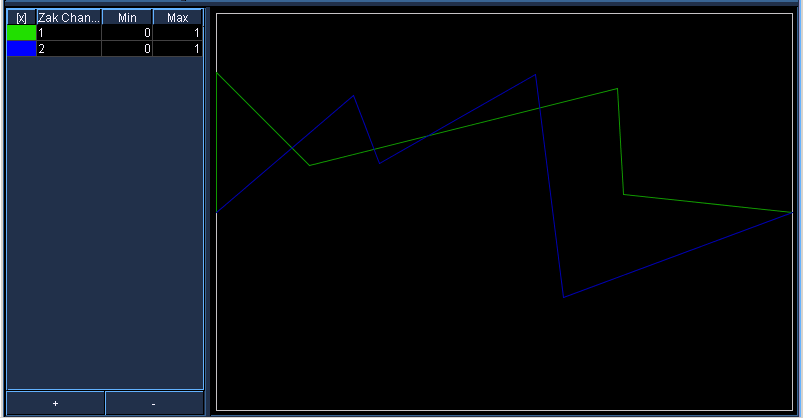
\includegraphics{images/zakLineObject.png}

Add and graphically edit zak k-rate signals.

Use the bottom + and - buttons to add/remove lines.

Use the left panel to select a line by clicking on the row describing
the line you wish to edit; you'll know which one is select by the edit
points showing up in the right panel showing the line. To edit the color
of the line, double click in the left panel on the color box to the left
of the "Zak Channel" column. A color selection dialog will appear for
the user to choose their desired color.

Enter the zak channel that you whish the signal to be written to under
the "Zak Channel" column. The "min" and "max" columns define the min and
max values of the graph that the line is drawn in to the right. However,
the min and max values can be different on a per-line basis.

When editing the line in the right panel, left clicking adds a point at
the current cursor position. Right-clicking will delete a point when a
point is under the cursor (you can easilly tell this because the a point
will change to red when the cursor is hovering over it). You can move a
point by left-clicking and dragging.

